%% \documentclass[twocolumn]{article}
\documentclass[pre,twocolumn,twoside,byrevtex,superscriptaddress]{revtex4}

\usepackage{amsmath}
\usepackage{amssymb}
\usepackage{url}
\usepackage{graphicx}
\usepackage{listings,color}
\usepackage{setspace}

\lstset{language=matlab,
        basicstyle=\ttfamily\scriptsize\singlespacing,
        keywordstyle=\color{blue},
        stringstyle=\color{red},
        commentstyle=\color{green},
        morecomment=[l][\color{magenta}]{\#},
        frame=L,
        xleftmargin=\parindent,
        numbersep=5pt,
        breaklines=true,
        breakatwhitespace=false,
        escapeinside={\%*}{*)},
}

\setlength{\parindent}{0cm}

\setlength{\parskip}{1mm}

\begin{document}

%% \twocolumn[
%%   \begin{@twocolumnfalse} 

%%     \title{\vspace{-2cm}Homework 4: Counterprop}
%%     \author{Andy Reagan}

%%     \maketitle

%%   \end{@twocolumnfalse}
%% ]

\title{\vspace{-2cm}Homework 6: GRNN}
\author{Andy Reagan}

\begin{abstract}
I code and discuss a Generalized Regression Nueral Network (GRNN) as described in 
\end{abstract}

\maketitle

\section{Introduction}

Originally proposed by Kohonen, the self organizing map describes a general class of unsupervised artificial nueral networks \cite{kohonen1990self}.
They can be run unsupervised, but in use as a classifier it is best to supervise a fine tuning process, and they become a semi-supervised process.

\begin{figure}
 \centering
  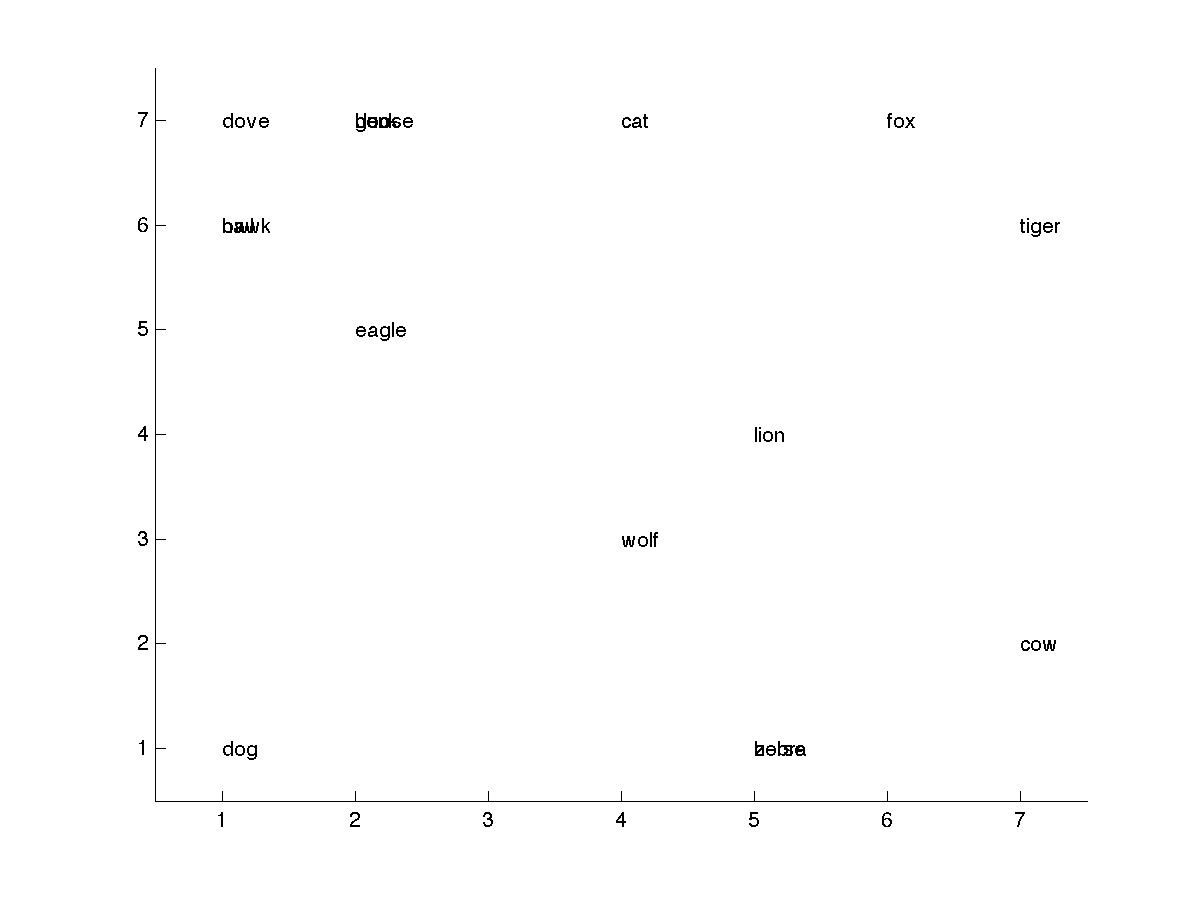
\includegraphics[width=0.48\textwidth]{../figures/animals-layout.png}
  \label{fig:1}
  \caption{Labels for different animals plotted over their closest Kohonen node.
The nodes are laid out on a square grid, which is like the topology of the network, which uses a Von Neumann neighborhood.
Some animals have the same attributes, and got plotted in the same place!}
\end{figure}



\section{Methods}

I closely follow the paper of Kohonen in coding up the SOM.
It is definitely tricky, but leading the paper discussion forced me to understand it a bit more.

Since I'm hoping to use this as a classifier in my project, I'm paid careful attention to this use case.
In particular, there are two ways to lay out the network.
The first, in displaying how the animals are classified, looks at the nodes of the network laid in space, by their topology.
The second lays out the nodes by their values, giving a better sense of the distribution which they are now approximating.

The big hang-up for my code is implementing the network topology, and changing the size of the neighborhood used in training.
I took the flat network, and built an adjacency matrix for it.
Then, based how far in the training we are, I travel this adjacency matrix for across a maximum path length.
My implementations of both of these concepts are definitely lacking.

Thinking about the network like a CA, it might be easier to use a matrix as the nodes and avoid the full adjacency matrix altogether.
This would definitely be faster.
But this approach in limited in the type of topology that is possible.

\section{Results}

I had no problems, over a variety of parameters, to do a reasonably good job separating out the types of animals.
Attempting to get the map to spread out over the uniform 2D distribution was more difficult.
My implementation is slow, so I was only able to run reasonably for 100 samples and a network of size 25.
It was sensitive to both the neighborhood decay and the decay of the learning parameter.
A decay that was too rapid in the learning parameter didn't give it enough time to spread out, and a deacy that was too slow let it spread out, then cluster again.
It was also important to keep the path length long initially, for it to spread out.
And if that doesn't decay quick enough, my code takes forever to run.

In the end, I think that the SOM is a lot of fun, and is definitely worthwhile for different applications.
But, you need to be careful about how to apply it, and how to interperet the results.
In particular, although it is ``unsupervised'', it's not a black box.
So, you still have to know what's going on, and be careful, like with the fully supervised learning that we've seen.

What follows is essentially restatement of what Kohonen says in his paper, and an inclusion of the equation for the Bayes classification, trying to make sense of how this works.
As a bayesian classifier, we write the conditional probability of the vector $x$ belonging to class $C_k$ as
\begin{equation}
  p(C_k|x) = \frac{p(C_k)p(x|C_k)}{p(x)}
\end{equation}
and, as Kohonen writes, the decision boundaries are where the function
\begin{equation}
  | p(C_i)p(x|C_i) - p(C_j)p(x|C_j) |
\end{equation}
eqauls 0.
So, by using the nearest neighbor choice for classification, this is akin to using the bayesian classifier
\begin{equation}
  k = \max_k p(C_k) \prod _i p(x_i|C_k)
\end{equation}
where we're choosing the $k$ such that our network nodes have the greatest density in $p(x_i|C_k)$.

\begin{figure}
 \centering
  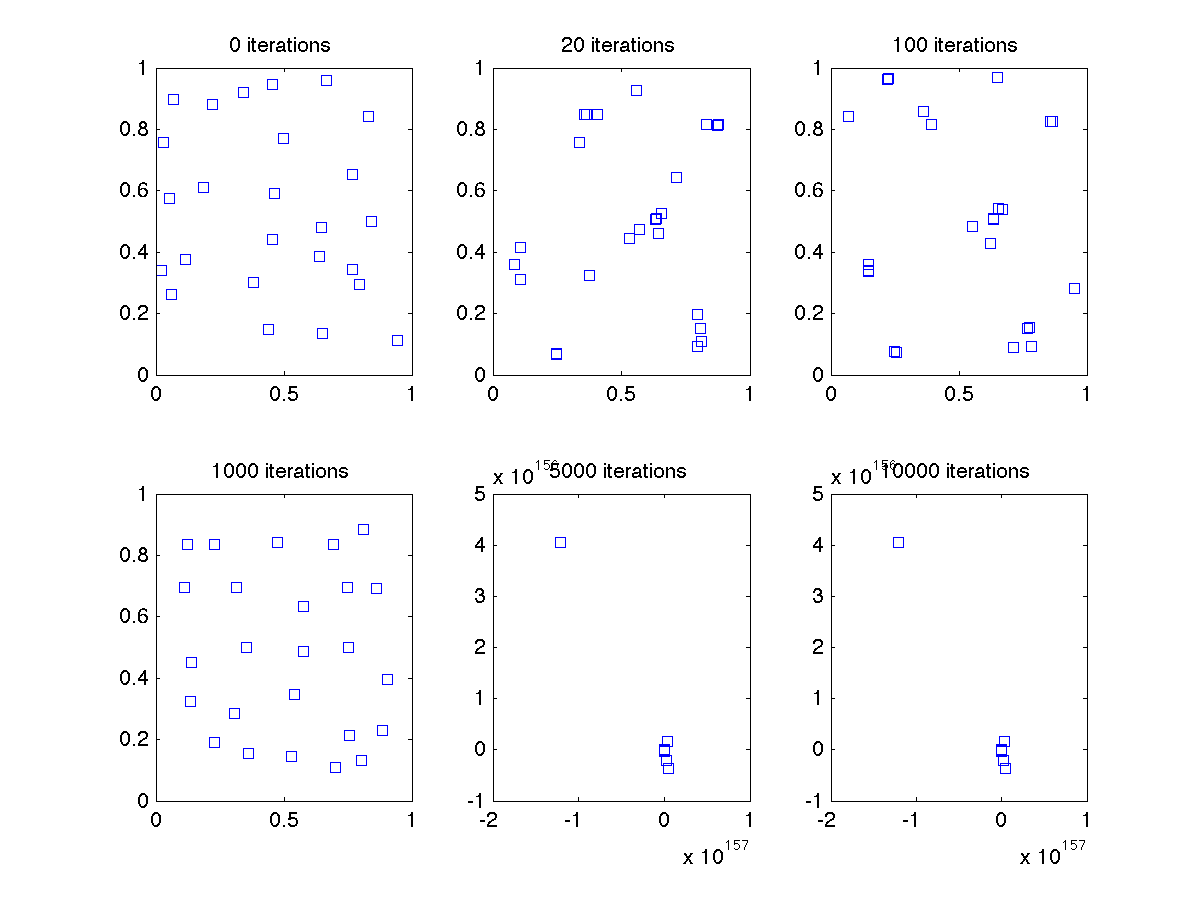
\includegraphics[width=0.48\textwidth]{figures/SOM_uniform_dist_covering_long.png}
  \label{fig:2}
  \caption{An example where the learning parameter decays too slowly. What looks like convergence is lost! Notice that the bounds on the final two plots grow to $10^5$.}
\end{figure}

\bibliographystyle{chicago}
\bibliography{writeup}

\clearpage
\pagebreak
\onecolumngrid

    \section*{Full code}

    \lstinputlisting{SOM_andy_driver.m}
    \lstinputlisting{train_SOM.m}
    \lstinputlisting{scaling_inverse.m}
    \lstinputlisting{moore_decaying.m}

%% \clearpage
%% \pagebreak

%%     \section*{Extra figures}

%%     %% \begin{figure}
%%     %%   \centering
%%     %%   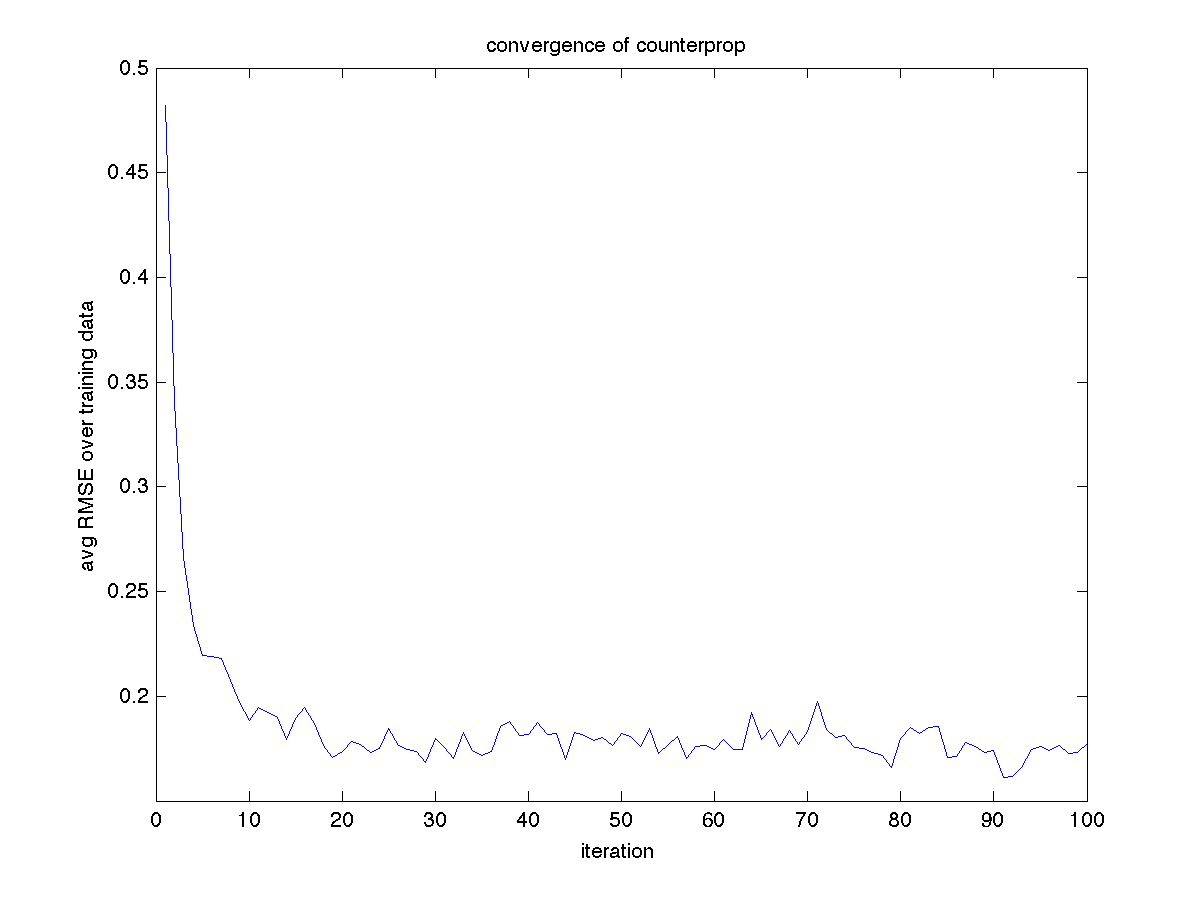
\includegraphics[width=0.68\textwidth]{111.png}
%%     %%   \label{fig:1}
%%     %%   \caption{Basic convergence test.}
%%     %% \end{figure}

\end{document}
